\documentclass[10pt]{article}
\usepackage[polish]{babel}
\usepackage[utf8]{inputenc}
\usepackage[T1]{fontenc}
\usepackage{amsmath}
\usepackage{amsfonts}
\usepackage{amssymb}
\usepackage[version=4]{mhchem}
\usepackage{stmaryrd}
\usepackage{graphicx}
\usepackage[export]{adjustbox}
\graphicspath{ {./images/} }

\title{1. Oblicz granicę ciągu }

\author{}
\date{}


\begin{document}
\maketitle
\[
\lim _{n \rightarrow \infty}\left(2 n-\sqrt[3]{8 n^{3}-2 n^{2}}\right)
\]

\begin{enumerate}
  \setcounter{enumi}{1}
  \item Oblicz \(\sqrt{\underbrace{44 \ldots 4}_{2 n}+\underbrace{11 \ldots 1}_{n+1}-\underbrace{66 \ldots 6}_{n}}\)
  \item Czerwony odcinek jest styczny do obu ćwiartek koła. Jaka część prostokąta jest zamalowana na zielono?\\
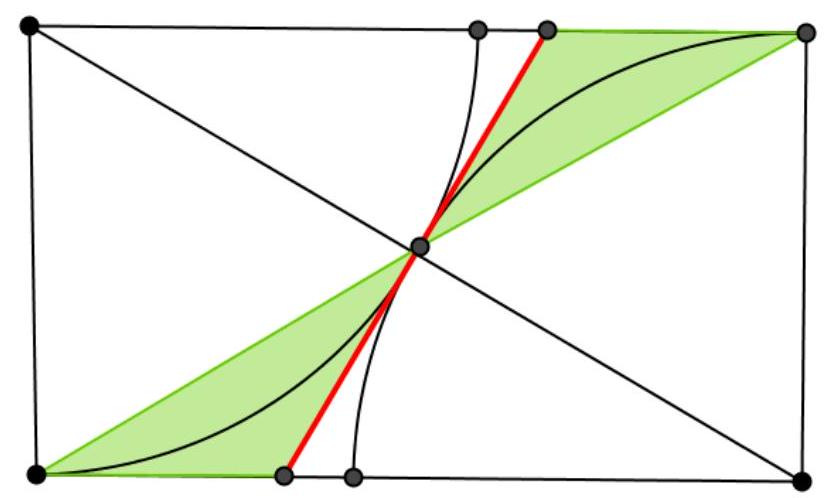
\includegraphics[max width=\textwidth, center]{2024_11_21_e6768d6d37bcac47327bg-1}
\end{enumerate}

\end{document}